\chapter{Introducción}

El catión Cobre(II), \ce{Cu^{2+}}, participa en una amplia y diversa gama de fenómenos, abarcando desde procesos biológicos esenciales hasta complejas interacciones químicas y aplicaciones tecnológicas de vanguardia. Su particular configuración electrónica $d^9$ le confiere propiedades estructurales y redox únicas que han sido objeto de numerosos estudios teóricos y experimentales.

\subsection*{Implicaciones en Sistemas Biológicos y la Salud Humana}

En el dominio de la bioquímica, el \ce{Cu^{2+}} es un micronutriente vital. Su función más prominente es como componente clave de numerosas metaloenzimas que catalizan procesos críticos, tales como el transporte de electrones y oxígeno —ejemplificado por la hemocianina— y la oxidación catalítica de sustratos orgánicos como fenoles y aminas \cite{Cu-2014-01, Wa-2024-03, Wa-2017-01, Wa-2009-01}. Adicionalmente, es fundamental para la movilización del hierro durante la síntesis de hemoglobina.

No obstante, la homeostasis del cobre es delicada. Desequilibrios en su concentración están directamente implicados en patologías graves. La regulación deficiente del cobre se ha conectado con trastornos neurodegenerativos como las enfermedades de Parkinson y Alzheimer \cite{Cu-2014-02,Cu-2011-02, Cu-2012-01}. Asimismo, los desequilibrios en los niveles de ceruloplasmina, que facilita el transporte de Cu2+ en el torrente sanguíneo, pueden provocar el síndrome de Menkes o la enfermedad de Wilson \cite{Cu-2001-01, Cu-2017-01}.

\subsection*{Aplicaciones en Catálisis}

Más allá de su rol biológico, los complejos de cobre son herramientas poderosas en la síntesis química y la tecnología. En el campo de la catálisis, son ampliamente utilizados para la construcción de enlaces carbono-carbono y carbono-heteroátomo, y son indispensables en reacciones como el acoplamiento de Sonogashira-Hagihara y la activación de enlaces C-H. El objetivo actual se centra en el desarrollo de catalizadores basados en cobre que no solo sean eficientes y selectivos, sino también respetuosos con el medio ambiente \cite{Cu-2014-01}.

\section{La Química de Coordinación Única del \ce{Cu^{2+}}: El Efecto Jahn-Teller}

La versatilidad fisicoquímica del catión cobre(II) (\ce{Cu^{2+}}) emana directamente de su estructura electrónica \ce{[Ar]}$d^9$ , siendo el fenómeno central que gobierna su comportamiento la distorsión de Jahn-Teller (JTE). Este efecto se manifiesta como una deformación geométrica espontánea que ocurre en moléculas no lineales con un estado electrónico fundamental degenerado. El teorema postula que el sistema reduce su simetría para eliminar dicha degeneración, lo que resulta en una disminución de su energía total \cite{Cu-2019-01}.

En un complejo octaédrico de \ce{Cu^{2+}}, la configuración \ce{[Ar]}$d^9$ presenta orbitales $e_g$ degenerados. La distorsión para resolver esta degeneración emerge de la diferencia en la densidad electrónica entre el metal y los ligandos  y puede presentarse de dos maneras:
\begin{itemize}
    \item \textbf{Elongación (z-out):} Los dos enlaces axiales se alargan y los cuatro ecuatoriales se acortan. Esto ocurre cuando la densidad electrónica es mayor en el eje $z$ y el orbital molecular semiocupado (SOMO por sus siglas en inglés) es el $d_{x^2-y^2}$.
    \item \textbf{Compresión (z-in):} Los cuatro enlaces ecuatoriales se alargan y los dos axiales se acortan. Sucede cuando la densidad electrónica es mayor en el plano $xy$ y el SOMO es el $d_{z^2}$.
\end{itemize}


\begin{figure}[H]
    \centering
    
    % Fila superior: Distorsión z-out (Elongación)
    \begin{subfigure}{0.2\textwidth}
        \centering
        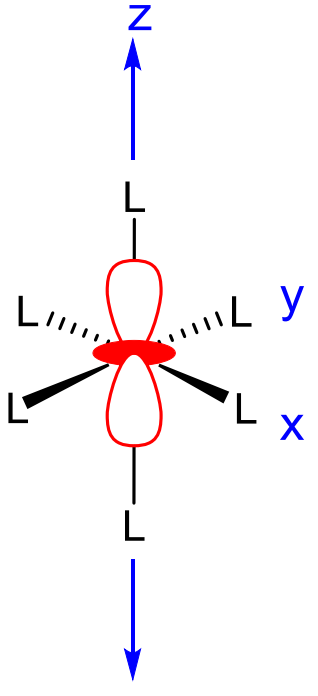
\includegraphics[width=0.5\linewidth]{Imágenes/JTE-z-out-draw.png}
        \caption{}
    \end{subfigure}
    %\hfill % Espacio horizontal entre imágenes
    \begin{subfigure}{0.2\textwidth}
        \centering
        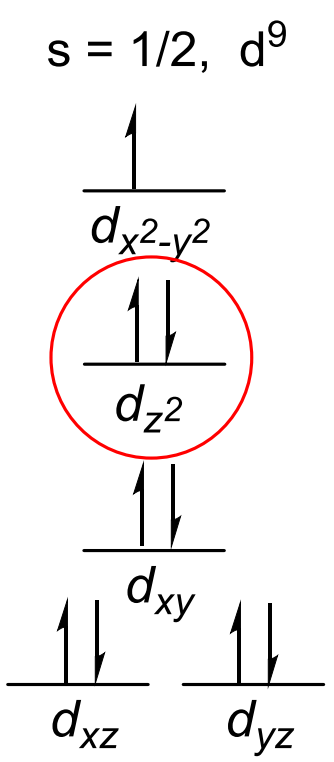
\includegraphics[width=0.5\linewidth]{Imágenes/JTE-z-out-orbitals.png}
        \caption{}
    \end{subfigure}
    
    \vspace{0.5cm} % Espacio vertical entre filas
    
    % Fila inferior: Distorsión z-in (Compresión)
    \begin{subfigure}{0.3\textwidth}
        \centering
        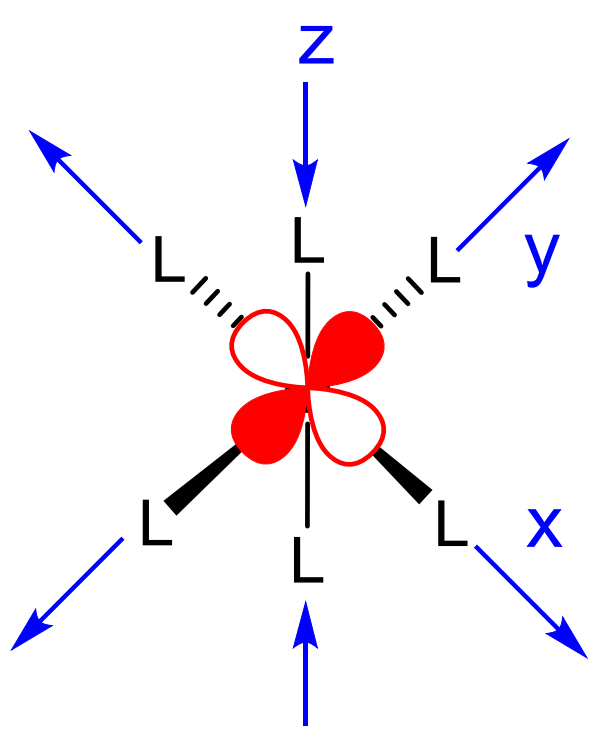
\includegraphics[width=0.5\linewidth]{Imágenes/JTE-z-in-draw.png}
        \caption{}
    \end{subfigure}
    %\hfill % Espacio horizontal entre imágenes
    \begin{subfigure}{0.2\textwidth}
        \centering
        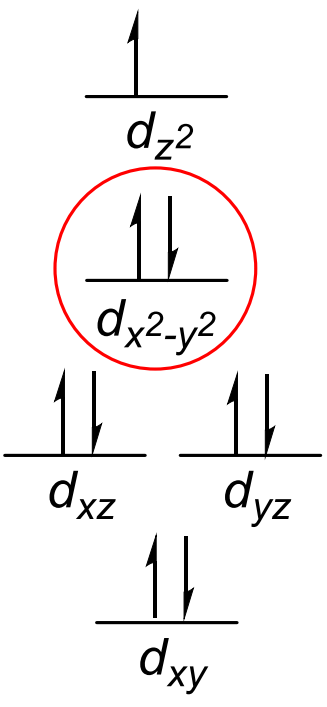
\includegraphics[width=0.5\linewidth]{Imágenes/JTE-z-in-orbitals.png}
        \caption{}
    \end{subfigure}
    
    \caption[Ilustración del efecto Jahn-Teller ]{Ilustración  del efecto Jahn-Teller para un complejo octaédrico del ion Cu(II) con configuración electrónica $d^9$. Arriba se muestra la distorsión por elongación axial (z-out), donde los enlaces axiales se alargan (a), y su correspondiente desdoblamiento de orbitales (b). Abajo se presenta la distorsión por compresión axial (z-in), con el acortamiento de los enlaces axiales (c) y su respectivo desdoblamiento energético (d). La distorsión z-out es la observada más comúnmente en la experimentación. Ilustración obtenida de la referencia \cite{Cu-2019-01}}
    \label{fig:jahn_teller_d9}
\end{figure}


Aunque la elongación es la geometría más común, estudios teóricos han demostrado que ambas son posibles para el catión \ce{[Cu(OH2)6]^{2+}} \cite{Cu-2019-01}.

El JTE no es un mero detalle, sino una de las principales causas de la química de coordinación excepcionalmente flexible y dinámica del \ce{Cu^{2+}}. Dota al ion de una plasticidad estructural inusual, permitiéndole adoptar múltiples geometrías (octaédrica distorsionada, piramidal cuadrada, planar cuadrada) con diferencias energéticas muy pequeñas entre ellas. Esta flexibilidad es inherentemente dinámica; en solución, el complejo interconvierte rápidamente entre estas configuraciones. Esto explica la alta labilidad de sus ligandos, cuya tasa de intercambio es órdenes de magnitud superior a la de otros cationes divalentes. La debilidad de los enlaces axiales facilita este rápido intercambio y ha generado un prolongado debate sobre el número de coordinación preferido (4, 5 o 6) del ion en solución.

\section{Hidratación}

\subsection*{Estudios Experimentales}

Históricamente, los estudios experimentales han sido la piedra angular en la comprensión de la solvatación del Cu\textsuperscript{2+}. Las técnicas más utilizadas incluyen:
\begin{itemize}
    \item Difracción de Rayos X y Neutrones
    \item Espectroscopia de Absorción de Rayos X (EXAFS y XANES)
\end{itemize}

Los primeros trabajos de difracción en las décadas de 1970 y 1980 establecieron la idea de una coordinación octaédrica distorsionada (NC=6), con una configuración (4+2) que implicaba cuatro ligandos de agua en posiciones ecuatoriales y dos más distantes en posiciones axiales \cite{Wa-1988-01}. Sin embargo, a partir del año 2000, estudios más avanzados, que combinaban técnicas como la difracción de neutrones con dinámica molecular o empleaban análisis de EXAFS y XANES más sofisticados, comenzaron a favorecer un modelo de coordinación quíntuple (NC=5) con una geometría de pirámide cuadrada \cite{Wa-2001-01, Wa-2002-01}.

Actualmente, existe un consenso experimental sobre las distancias de enlace ecuatoriales ($Cu-O_{eq}$), que se reportan consistentemente en el rango de 1.93--2.01 \AA. Por el contrario, las distancias axiales ($Cu-O_{ax}$) son más difíciles de medir y presentan una mayor variabilidad, con valores que oscilan entre 2.15 \AA \ y 2.60 \AA. Investigaciones recientes de alta resolución sugieren incluso la existencia de dos distancias axiales distintas, lo que apunta a un octaedro no centrosimétrico. Algunos estudios que emplean un enfoque multitécnica han llegado a proponer un NC promedio de 4.5, lo que refuerza la idea de una mezcla dinámica de geometrías en solución. La imagen moderna, por tanto, describe una "plasticidad estructural" donde múltiples estados de coordinación coexisten en un equilibrio dinámico. El resumen de todos estos trabajos se encuentra en la tabla \ref{tab:agua-paramteros-estructurales-experimentales-y-teoricos}.

\subsection*{Estudios Teóricos}

Los estudios computacionales han sido fundamentales para interpretar la evidencia experimental y proporcionar una visión dinámica del proceso de solvatación. Los principales métodos teóricos empleados son:
\begin{itemize}
    \item Teoría del Funcional de la Densidad (DFT)
    \item Dinámica Molecular (MD), tanto clásica como \textit{ab initio} (AIMD)
    \item Métodos híbridos de Mecánica Cuántica/Mecánica Molecular (QM/MM)
\end{itemize}

Las simulaciones teóricas corroboran la naturaleza dinámica del efecto Jahn-Teller, mostrando transformaciones rápidas entre diferentes configuraciones en escalas de tiempo de femtosegundos. Gran parte de los modelos teóricos indican que la geometría de pirámide cuadrada (NC=5) es la más estable en solución acuosa, aunque la diferencia de energía con la forma hexa-coordinada (NC=6) es muy pequeña ($\sim$1.4 kcal/mol) \cite{Wa-2008-01, Wa-2009-02}. Esto sugiere que ambas especies pueden coexistir en solución, lo cual está en línea con los hallazgos experimentales.

Un aporte crucial de los estudios teóricos ha sido resaltar el papel de la segunda capa de solvatación. Se ha demostrado que la formación de enlaces de hidrógeno entre las moléculas de agua de la primera y segunda esfera de hidratación es un factor de estabilización que puede competir energéticamente con la coordinación de una molécula de agua en la posición axial \cite{Wa-2007-03, Wa-2008-01,Wa-2024-01}. Las distancias de enlace calculadas concuerdan bien con los datos experimentales, con valores promedio para $Cu-O_{eq}$ de alrededor de 2.00--2.03 \AA \ y para $Cu-O_{ax}$ de 2.15--2.30 \AA. El resumen de todos estos trabajos también se encuentra en la tabla \ref{tab:agua-paramteros-estructurales-experimentales-y-teoricos}.

\section{Solvatación  en Metanol}


Al igual que en el agua, la estructura de solvatación del ion \ce{Cu^{2+}} en metanol es un área de investigación activa, aunque la cantidad de estudios disponibles es notablemente más escasa. Dada la inherente naturaleza dinámica de la primera esfera de coordinación documentada para el fenómeno de hidratación, la solvatación en medio metanólico también presenta un debate sobre el número de coordinación (NC) y la geometría predominantes, con diferentes estudios experimentales y teóricos llegando a conclusiones diversas.

\subsection*{Estudios Experimentales}

Las investigaciones experimentales han empleado diversas técnicas espectroscópicas para determinar la estructura local del Cu\textsuperscript{2+} en metanol. Entre los métodos más destacados se encuentran:
\begin{itemize}
    \item Espectroscopia de absorción de rayos X (EXAFS y XANES)
    \item Análisis de modulación de eco de espín de electrones
    \item Estudios de Resonancia Magnética Nuclear (RMN) de Oxígeno-17
\end{itemize}

El panorama experimental se caracteriza por una falta de acuerdo. Mientras que estudios tempranos \cite{Me-1980-01} propusieron una coordinación de seis (NC=6), trabajos posteriores sugirieron que la técnica empleada podría haber sobrestimado las distancias de enlace. Más tarde, estudios de RMN \cite{Me-1986-01} observaron una "rápida transición" de isómeros hexacoordinados a conformaciones de cinco coordinaciones (NC=5), introduciendo la idea de un equilibrio dinámico.

Este debate continúa en estudios más recientes. Por un lado, en un estudio que combina EXAFS y XANES concluyeron \char"22 inequívocamente\char"22 \ que el \ce{Cu^{2+}} en metanol adopta una geometría de pirámide cuadrada con NC=5 \cite{Me-2012-01}. Por otro lado, un estudio más reciente con EXAFS de alta calidad determinó que el mejor modelo de ajuste correspondía a una estructura octaédrica distorsionada por Jahn-Teller con NC=6 y carácter no centrosimétrico \cite{Wa-2020-01}, contradiciendo directamente la conclusión anterior.

A pesar de la discrepancia en el NC, hay un mayor consenso en las distancias de enlace ecuatoriales ($Cu-O_{eq}$), reportadas consistentemente en el rango de 1.95--1.98 \AA. Las distancias axiales ($Cu-O_{ax}$), sin embargo, varían más, con valores reportados de 2.23 \AA \ para el modelo de NC=5 y dos distancias distintas de aproximadamente 2.20 \AA \ y 2.34 \AA \ para el modelo de NC=6. El resumen de dichos trabajos se encuentra en la tabla \ref{tab:metanol-paramteros-estructurales-experimentales-y-teoricos}.

\subsection*{Estudios Teóricos}

Los métodos computacionales han sido cruciales para explorar el complejo panorama energético de la solvatación del Cu\textsuperscript{2+} en metanol. Las principales técnicas utilizadas incluyen:
\begin{itemize}
    \item Métodos \textit{ab initio} como MP2 
    \item Teoría del Funcional de la Densidad (DFT), en particular con el funcional M06-2X
    \item Modelos de disolvente continuo implícito (IEF-PCM)
\end{itemize}

Los estudios teóricos, principalmente los trabajos exhaustivos de Da-yang et al., han demostrado que el NC más estable depende fuertemente de las condiciones del modelo, como el tamaño del clúster de solvente (n), la temperatura y el entorno (fase gaseosa vs. disolvente implícito).

En la fase gaseosa, los cálculos muestran una competencia entre diferentes números de coordinación. El método MP2 tiende a favorecer isómeros tetra- y pentacoordinados \cite{Me-2022-01}, mientras que el método DFT (M06-2X) favorece a los penta- y hexacoordinados \cite{Me-2023-01}. Para clústeres pequeños (n=1-5), las coordinaciones más bajas son las más estables, pero a medida que aumenta el tamaño, las estructuras de mayor NC ganan relevancia.

La inclusión de un modelo de disolvente implícito (IEF-PCM) tiene un impacto discernible y cambia el panorama. En este entorno, se observa una clara preferencia por los números de coordinación más altos, desfavoreciendo a las estructuras de NC=4. Para clústeres de mayor tamaño (n=7-10), las estructuras hexacoordinadas (NC=6) dominan exclusivamente la población a cualquier temperatura \cite{Me-2023-02}. Este hallazgo subraya la importancia crítica del efecto del medio dieléctrico para estabilizar geometrías más compactas y con mayor número de coordinación.

Las distancias de enlace calculadas teóricamente muestran una excelente concordancia con los datos experimentales, con valores de $Cu-O_{eq}$ que oscilan entre 1.94--2.02 \AA \ y de $Cu-O_{ax}$ entre 2.15 -- 2.27 \AA. Los cálculos también revelan que el disolvente alarga los enlaces dativos axiales en las estructuras pentacoordinadas en comparación con la fase gaseosa.



\section{Justificación y Enfoque Metodológico}

Históricamente, los métodos experimentales como la difracción de rayos X y neutrones o las espectroscopias EXAFS y XANES han sido cruciales para sondear estos sistemas. Sin embargo, a pesar de su capacidad para medir distancias de enlace con precisión, estos métodos enfrentan limitaciones significativas. A menudo existe una considerable controversia y ambigüedad en la determinación del número de coordinación (NC) y la geometría, y resulta técnicamente difícil distinguir entre estructuras con energías muy similares, como las de coordinación cuádruple, quíntuple y séxtuple, que pueden coexistir en solución.

Frente a estas limitaciones, los métodos teóricos y las simulaciones computacionales emergen como una herramienta indispensable. Enfoques como la Dinámica Molecular (MD) basada en la Teoría del Funcional de la Densidad (DFT) permiten superar las desventajas experimentales al proporcionar una visión detallada a nivel atómico. Estos métodos posibilitan la exploración de superficies de energía potencial, la caracterización de efectos dinámicos como la inversión del eje de Jahn-Teller en escalas de tiempo de picosegundos, y el estudio de interacciones complejas como la transferencia de carga y los enlaces de hidrógeno, que son difíciles de aislar experimentalmente. Si bien los métodos teóricos no están exentos de desventajas, como el alto costo computacional y una fuerte sensibilidad a la elección del funcional y la base de conjunto, su capacidad para modelar la dinámica y la coexistencia de múltiples estados los convierte en una opción poderosa para resolver las controversias existentes.

El presente trabajo de tesis aprovecha las ventajas de los métodos teóricos para abordar dos frentes. 

\begin{itemize}
    \item Primero, se estudia la solvatación del \ce{Cu^{2+}} en metanol, un área donde la información experimental y teórica es notablemente más escasa en comparación con el agua. Este vacío de conocimiento representa un área de oportunidad significativa. Por ello, este trabajo presenta por primera vez en la literatura un estudio teórico  basado en dinámica molecular \textit{ab initio} (BOMD por sus siglas en inglés) sobre la estructura y dinámica de los clústeres de \ce{[Cu(CH_3OH)_40]^{2+}} utilizando DFT/M06-2X.
    \item  Segundo, se reexamina el sistema acuoso (\ce{[Cu(H_2O)_40]^{2+}}. A pesar de ser un caso extensamente estudiado, la mayoría de los trabajos teóricos previos han empleado la dinámica molecular de Car-Parrinello y funcionales de tipo GGA (como BLYP y PBE). Aunque dichos enfoques han sido fundamentales, poseen limitaciones intrínsecas bien conocidas para describir la compleja estructura electrónica del cobre (II) y sus interacciones no covalentes.
\end{itemize}

El trabajo aprovecha los avances en DFT al utilizar el funcional de intercambio y correlación M06-2X. Al ser un funcional altamente parametrizado para interacciones no covalentes y metales de transición \cite{DFT-2008-01} nos permite modelar con una fidelidad cuántica superior la sutil competencia entre la coordinación en la primera esfera y la estabilización por enlaces de hidrógeno de la segunda. Adicionalmente, se ha demostrado que el funcional M06-2X es una alternativa computacionalmente eficiente a métodos \textit{ab initio} computacionalmente más costosos como el MP2 y ha demostrado un buen rendimiento al describir sistemas similares de cationes de metales de transición en medios polares.

En los siguientes capítulos se expondrá el marco teórico detallado de la Dinámica Molecular y la Teoría del Funcional de la Densidad, explicando la naturaleza del funcional M06-2X. Posteriormente, se presentará la metodología computacional empleada para la construcción y simulación de los sistemas en ambos disolventes. Finalmente, se realizará un análisis exhaustivo de los resultados y se presentarán las conclusiones derivadas de este estudio.
